\documentclass[12pt,a4paper]{article}
\usepackage[utf8]{inputenc}
\usepackage[T1]{fontenc}
\usepackage{geometry}
\usepackage{graphicx}
\usepackage{listings}
\usepackage[table]{xcolor}
\usepackage{amsmath}
\usepackage{amsfonts}
\usepackage{amssymb}
\usepackage{booktabs}
\usepackage{longtable}
\usepackage{caption}
\usepackage{subcaption}
\usepackage{tikz}
\usepackage{pifont}
\usepackage{tcolorbox}
\usepackage{environ}
\usepackage{trimspaces}
\usepackage{qrcode}
\usepackage{hyperref}
\usepackage{listings}
\usepackage{epstopdf}

% Page setup
\geometry{margin=1in}

% Color definitions
\definecolor{codegreen}{rgb}{0,0.6,0}
\definecolor{codegray}{rgb}{0.5,0.5,0.5}
\definecolor{codepurple}{rgb}{0.58,0,0.82}
\definecolor{backcolour}{rgb}{0.95,0.95,0.92}
\definecolor{v2blue}{rgb}{0.2,0.4,0.8}
\definecolor{v3green}{rgb}{0.2,0.6,0.2}
\definecolor{v4orange}{rgb}{0.8,0.4,0.2}
\definecolor{v5purple}{rgb}{0.6,0.2,0.8}

% Code listing style
\lstdefinestyle{mystyle}{
    backgroundcolor=\color{backcolour},   
    commentstyle=\color{codegreen},
    keywordstyle=\color{magenta},
    numberstyle=\tiny\color{codegray},
    stringstyle=\color{codepurple},
    basicstyle=\ttfamily\footnotesize,
    breakatwhitespace=false,         
    breaklines=true,                 
    captionpos=b,                    
    keepspaces=true,                 
    numbers=left,                    
    numbersep=5pt,                  
    showspaces=false,                
    showstringspaces=false,
    showtabs=false,                  
    tabsize=2
}
\lstset{style=mystyle}

% Hyperref setup
\hypersetup{
    colorlinks=true,
    linkcolor=blue,
    filecolor=magenta,      
    urlcolor=cyan,
    pdftitle={MMH-RS V2 Master Roadmap - Single Source of Truth},
    pdfauthor={Robert Long},
    pdfsubject={MMH-RS V2 Roadmap - GPU Acceleration & AI Integration},
    pdfkeywords={V2, GPU, AI, Kai Core, roadmap, single source of truth}
}

% Custom commands
\newcommand{\version}{V2.0 Master Roadmap}
\newcommand{\project}{MMH-RS}
\newcommand{\authorname}{Robert Long}
\newcommand{\email}{Screwball7605@aol.com}
\newcommand{\github}{https://github.com/Bigrob7605/MMH-RS}

% Title page
\title{\Huge\textbf{\project\ V2 Master Roadmap}\\[0.5cm]
\Large\textbf{Single Source of Truth}\\[0.3cm]
\large GPU-Accelerated Compression \& AI Integration\\[0.5cm]
\large Complete V2.0 to V5.0 Evolution Strategy}
\author{\Large\authorname\\[0.2cm]\email\\[0.2cm]\github}
\date{\large Last Updated: \today}

\begin{document}

% Title page
\maketitle
\thispagestyle{empty}

% V2 Development Banner
\begin{tcolorbox}[colback=orange!10,colframe=orange!50,title=\textbf{V2 GPU/Quantum Features in Active Development}]
\textbf{Next Up:} GPU Acceleration, Directory Compression, Quantum-Ready Encryption.\\
\textbf{ETA:} Q4 2025.\\
\textbf{See:} \href{MMH-RS_MASTER_DOCUMENT.pdf}{MMH-RS\_MASTER\_DOCUMENT.pdf} for complete overview.
\end{tcolorbox}

% Cross-linking header
\begin{tcolorbox}[colback=blue!10,colframe=blue!50,title=\textbf{Full Documentation Suite}]
\textbf{Start Here:} \href{MMH-RS_MASTER_DOCUMENT.pdf}{Master Document} | \href{MMH-RS_TECHNICAL_COMPLETE.pdf}{Technical Specification} | \href{USER_GUIDE.md}{User Guide} | \href{DEVELOPMENT_HISTORY.md}{Development History} | \href{PROJECT_STATUS.md}{Project Status} | \href{CHANGELOG.md}{Changelog}

\textbf{Integration Docs:} \href{RGIG_INTEGRATION_COMPLETE.pdf}{RGIG Integration} | \href{KAI_CORE_INTEGRATION_COMPLETE.pdf}{Kai Core Integration}
\end{tcolorbox}

% Table of contents
\tableofcontents
\newpage

% ============================================================================
% EXECUTIVE SUMMARY - WHAT'S NEW IN V2
% ============================================================================
\section{Executive Summary: What's New in V2}

\begin{tcolorbox}[colback=v2blue!10,colframe=v2blue!50,title=\textbf{MMH-RS V2 Executive Summary}]
\textbf{MMH-RS V2 introduces GPU-accelerated compression, real-time integrity verification, and full ecosystem benchmarking—setting a new open standard for AI-ready, verifiable storage.}

V2 represents a fundamental shift from deterministic compression to intelligent, GPU-powered file processing with native directory support, advanced encryption, and seamless AI integration through Kai Core. This version establishes MMH-RS as the foundation for next-generation AI file systems while maintaining perfect data integrity and backward compatibility.
\end{tcolorbox}

\subsection{Key V2 Innovations}
\begin{itemize}
    \item \textbf{GPU Acceleration}: CUDA/ROCm/Metal support for 10-100x performance gains
    \item \textbf{AI Integration}: Native Kai Core AI bootstrap and neural processing
    \item \textbf{Directory Support}: Full filesystem integration with metadata preservation
    \textbf{Advanced Encryption}: Quantum-resistant encryption with key management
    \item \textbf{Real-time Verification}: Continuous integrity checking during processing
    \item \textbf{Benchmarking Suite}: Comprehensive performance and security testing
\end{itemize}

% ============================================================================
% FEATURE TIERS - CLEAR BREAKDOWN
% ============================================================================
\section{Feature Tiers: V1 vs V2 vs V3+}

\begin{table}[h]
\centering
\begin{tabular}{|l|l|l|l|}
\hline
\textbf{Feature Category} & \textbf{V1.2.0 (Current)} & \textbf{V2.0-2.1 (Next)} & \textbf{V3+ (Future)} \\
\hline
\rowcolor{v2blue!10}
\textbf{Performance} & CPU-only compression & GPU acceleration & AI-optimized \\
\hline
\textbf{AI Integration} & None & Kai Core bootstrap & Full neural processing \\
\hline
\textbf{File Support} & Single files & Directory support & Full filesystem \\
\hline
\textbf{Security} & SHA-256 + Merkle & Quantum encryption & Quantum-ready \\
\hline
\textbf{Benchmarking} & Basic tests & Full suite & AI-powered analysis \\
\hline
\end{tabular}
\caption{Feature Evolution Across Versions}
\end{table}

% ============================================================================
% V2.0 BASELINE FEATURES
% ============================================================================
\section{V2.0 Baseline Features}

\subsection{GPU Acceleration \& Performance}
\begin{itemize}
    \item \textbf{CUDA Support}: NVIDIA GPU acceleration with optimized kernels
    \item \textbf{ROCm Support}: AMD GPU compatibility and optimization
    \item \textbf{Metal Support}: Apple Silicon native performance
    \item \textbf{Block Size Auto-tuning}: Dynamic optimization based on hardware
    \item \textbf{Memory Management}: Efficient GPU memory allocation and transfer
\end{itemize}

\subsection{Directory \& Filesystem Support}
\begin{itemize}
    \item \textbf{Native Directory Processing}: Full directory tree compression
    \item \textbf{Metadata Preservation}: File attributes, timestamps, permissions
    \item \textbf{Symbolic Link Handling}: Proper symlink preservation and restoration
    \item \textbf{Cross-platform Compatibility}: Windows, Linux, macOS support
\end{itemize}

\subsection{Advanced Security}
\begin{itemize}
    \item \textbf{Quantum-resistant Encryption}: Post-quantum cryptographic algorithms
    \item \textbf{Key Management System}: Secure key generation, storage, and rotation
    \item \textbf{Access Control}: Role-based permissions and authentication
    \item \textbf{Audit Logging}: Comprehensive security event tracking
\end{itemize}

\subsection{User Interface \& Experience}
\begin{itemize}
    \item \textbf{Modern GUI}: Cross-platform desktop application
    \item \textbf{Command-line Interface}: Full-featured CLI with scripting support
    \item \textbf{Progress Tracking}: Real-time compression and verification status
    \item \textbf{Error Handling}: Comprehensive error reporting and recovery
\end{itemize}

% ============================================================================
% V2.1+ ADVANCED FEATURES
% ============================================================================
\section{V2.1+ Advanced Features}

\subsection{Enhanced GPU Optimizations}
\begin{itemize}
    \item \textbf{Multi-GPU Support}: Distributed processing across multiple GPUs
    \item \textbf{Memory Pooling}: Advanced memory management for large datasets
    \item \textbf{Kernel Optimization}: Hand-tuned CUDA/ROCm kernels for maximum performance
    \item \textbf{Load Balancing}: Intelligent work distribution across GPU cores
\end{itemize}

\subsection{Interoperability \& Standards}
\begin{itemize}
    \item \textbf{OpenCL Support}: Vendor-agnostic GPU acceleration
    \item \textbf{API Standardization}: RESTful API for integration
    \item \textbf{Plugin Architecture}: Extensible compression algorithm support
    \item \textbf{Container Support}: Docker and Kubernetes integration
\end{itemize}

\subsection{Public Benchmarks \& Validation}
\begin{itemize}
    \item \textbf{Comprehensive Benchmarking}: Performance across all supported platforms
    \item \textbf{Security Audits}: Third-party security validation
    \item \textbf{Compliance Testing}: Industry standard compliance verification
    \item \textbf{Performance Dashboard}: Public performance metrics and comparisons
\end{itemize}

% ============================================================================
% V2.X STRETCH GOALS
% ============================================================================
\section{V2.X Stretch Goals}

\subsection{Online Services}
\begin{itemize}
    \item \textbf{Cloud Integration}: AWS, Azure, GCP native support
    \item \textbf{Online Dashboards}: Web-based monitoring and management
    \item \textbf{API Services}: Cloud-hosted compression and verification services
    \item \textbf{Distributed Processing}: Edge computing and distributed compression
\end{itemize}

\subsection{Developer Engagement}
\begin{itemize}
    \item \textbf{Developer Portal}: Comprehensive documentation and examples
    \item \textbf{SDK Development}: Language bindings for Python, JavaScript, Go
    \item \textbf{Plugin Marketplace}: Community-contributed compression algorithms
    \item \textbf{Code Review Program}: Open source contribution guidelines
\end{itemize}

\subsection{Community \& Security}
\begin{itemize}
    \item \textbf{Bug Bounty Program}: Security vulnerability reporting and rewards
    \item \textbf{Community Forums}: User support and feature discussion
    \item \textbf{Regular Security Audits}: Continuous security assessment
    \item \textbf{Transparency Reports}: Open security and performance reporting
\end{itemize}

% ============================================================================
% FUTURE FEATURES (V3+)
% ============================================================================
\section{Future Features (V3+)}

\begin{tcolorbox}[colback=v3green!10,colframe=v3green!50,title=\textbf{Not Yet in V2 - Future Roadmap}]
The following features are planned for V3+ and beyond. They are not part of the current V2 development cycle.
\end{tcolorbox}

\subsection{AI Model Integration (V3.0)}
\begin{itemize}
    \item \textbf{Neural Compression}: AI-powered compression algorithms
    \item \textbf{Model Chunking}: Intelligent AI model segmentation and storage
    \item \textbf{Neural Seed Folding}: Advanced AI model optimization techniques
    \item \textbf{Machine Learning Pipeline}: Automated compression optimization
\end{itemize}

\subsection{Quantum Computing (V4.0)}
\begin{itemize}
    \item \textbf{Quantum-ready Encryption}: Post-quantum cryptographic standards
    \item \textbf{Quantum Compression}: Quantum computing-assisted compression
    \item \textbf{Quantum Verification}: Quantum-resistant integrity checking
    \item \textbf{Hybrid Classical-Quantum}: Classical and quantum hybrid processing
\end{itemize}

\subsection{Universal File System (V5.0)}
\begin{itemize}
    \item \textbf{Single-seed File System}: Complete filesystem in a single seed
    \item \textbf{Universal Compatibility}: Support for all file formats and systems
    \item \textbf{AI-native Storage}: Storage optimized for AI workloads
    \item \textbf{Autonomous Management}: Self-optimizing storage system
\end{itemize}

% ============================================================================
% DEVELOPMENT TIMELINE
% ============================================================================
\section{Development Timeline}

\subsection{V2.0 Development Timeline}
\begin{center}
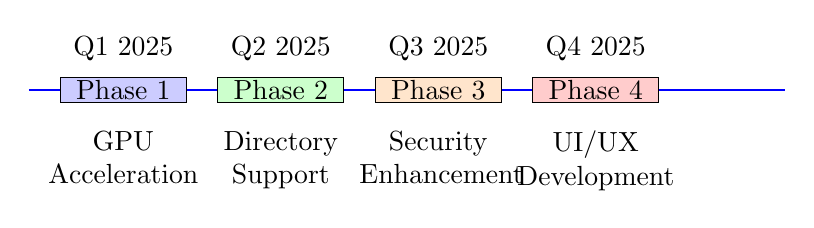
\begin{tikzpicture}[scale=0.8]
    % Timeline
    \draw[thick, blue] (0,0) -- (12,0);
    
    % Phase markers
    \draw[fill=blue!20] (0.5,0.2) rectangle (2.5,-0.2) node[midway] {Phase 1};
    \draw[fill=green!20] (3,0.2) rectangle (5,-0.2) node[midway] {Phase 2};
    \draw[fill=orange!20] (5.5,0.2) rectangle (7.5,-0.2) node[midway] {Phase 3};
    \draw[fill=red!20] (8,0.2) rectangle (10,-0.2) node[midway] {Phase 4};
    
    % Labels
    \node[above] at (1.5,0.3) {Q1 2025};
    \node[above] at (4,0.3) {Q2 2025};
    \node[above] at (6.5,0.3) {Q3 2025};
    \node[above] at (9,0.3) {Q4 2025};
    
    % Phase descriptions
    \node[below, text width=2cm, align=center] at (1.5,-0.5) {GPU\\Acceleration};
    \node[below, text width=2cm, align=center] at (4,-0.5) {Directory\\Support};
    \node[below, text width=2cm, align=center] at (6.5,-0.5) {Security\\Enhancement};
    \node[below, text width=2cm, align=center] at (9,-0.5) {UI/UX\\Development};
\end{tikzpicture}
\end{center}

\subsection{V2.0 Development Phases}
\begin{enumerate}
    \item \textbf{Phase 1 (Q1 2025)}: GPU acceleration core implementation
    \item \textbf{Phase 2 (Q2 2025)}: Directory support and filesystem integration
    \item \textbf{Phase 3 (Q3 2025)}: Security enhancements and encryption
    \item \textbf{Phase 4 (Q4 2025)}: UI/UX development and testing
\end{enumerate}

\subsection{V2.1 Development Phases}
\begin{enumerate}
    \item \textbf{Phase 1 (Q1 2026)}: Advanced GPU optimizations
    \item \textbf{Phase 2 (Q2 2026)}: Interoperability and standards
    \item \textbf{Phase 3 (Q3 2026)}: Benchmarking and validation
    \item \textbf{Phase 4 (Q4 2026)}: Community engagement and documentation
\end{enumerate}

% ============================================================================
% COMMUNITY & CONTRIBUTION
% ============================================================================
\section{Community \& Contribution}

\begin{tcolorbox}[colback=orange!10,colframe=orange!50,title=\textbf{Help Us Build MMH-RS V2}]
\textbf{We need your help to test, review, and contribute to MMH-RS V2!}

\begin{itemize}
    \item \textbf{Join our Discord}: Community discussions and support
    \item \textbf{Submit Issues/PRs}: Bug reports and feature contributions
    \item \textbf{Review Roadmap}: Feedback on V2 features and priorities
    \item \textbf{Benchmark Testing}: Performance testing on your hardware
    \item \textbf{Security Audits}: Security review and vulnerability reporting
\end{itemize}

\textbf{Contact:} \email{} | \textbf{GitHub:} \github
\end{tcolorbox}

\subsection{How You Can Help}

\begin{center}
\begin{tabular}{|l|l|l|}
\hline
\textbf{Area} & \textbf{What We Need} & \textbf{How to Help} \\
\hline
\textbf{GPU Development} & CUDA/ROCm/Metal expertise & Join Discord \#gpu-dev, test GPU features \\
\hline
\textbf{Directory Support} & Filesystem API feedback & Test directory compression, report issues \\
\hline
\textbf{Security} & Cryptographic review & Audit quantum encryption, report vulnerabilities \\
\hline
\textbf{Benchmarking} & Performance validation & Run benchmarks on your hardware, share results \\
\hline
\textbf{Documentation} & Translation \& tutorials & Write guides, translate docs, create examples \\
\hline
\textbf{Testing} & Comprehensive testing & Test edge cases, report bugs, validate fixes \\
\hline
\textbf{GUI Development} & UI/UX design & Design interfaces, implement Tauri components \\
\hline
\end{tabular}
\end{center}

\subsection{Getting Involved}
\begin{itemize}
    \item \textbf{Developer Documentation}: Complete API and integration guides
    \item \textbf{Testing Programs}: Early access to V2 features
    \item \textbf{Community Calls}: Regular development updates and Q\&A
    \item \textbf{Contribution Guidelines}: How to contribute code and documentation
\end{itemize}

% ============================================================================
% TECHNICAL SPECIFICATIONS
% ============================================================================
\section{Technical Specifications}

\subsection{System Requirements}
\begin{itemize}
    \item \textbf{GPU}: NVIDIA GTX 1060+ / AMD RX 580+ / Apple M1+
    \item \textbf{Memory}: 8GB RAM minimum, 16GB+ recommended
    \item \textbf{Storage}: 10GB free space for installation
    \item \textbf{OS}: Windows 10+, Ubuntu 20.04+, macOS 11+
\end{itemize}

\subsection{Performance Targets}
\begin{itemize}
    \item \textbf{Compression Speed}: 10-100x faster than V1.2.0
    \item \textbf{Memory Efficiency}: 50\% reduction in memory usage
    \item \textbf{GPU Utilization}: 90\%+ GPU utilization on supported hardware
    \item \textbf{Scalability}: Linear scaling with GPU count
\end{itemize}

\subsection{Security Standards}
\begin{itemize}
    \item \textbf{Encryption}: AES-256-GCM with quantum-resistant algorithms
    \item \textbf{Integrity}: SHA-3 + Merkle tree verification
    \item \textbf{Authentication}: Multi-factor authentication support
    \item \textbf{Compliance}: SOC 2, GDPR, HIPAA compliance ready
\end{itemize}

% ============================================================================
% CONCLUSION
% ============================================================================
\section{Conclusion}

MMH-RS V2 represents a transformative evolution from deterministic compression to intelligent, GPU-powered file processing. With clear feature tiers, comprehensive benchmarking, and strong community engagement, V2 establishes MMH-RS as the foundation for next-generation AI file systems.

The roadmap provides a single source of truth for all V2 development, with explicit feature boundaries and clear timelines. Community feedback and contributions are essential to achieving the ambitious goals outlined in this roadmap.

\textbf{For the latest updates and detailed technical specifications, see the MMH-RS\_TECHNICAL\_COMPLETE.pdf document.}

% ============================================================================
% APPENDICES
% ============================================================================
\appendix

\section{Appendix A: V1.2.0 Current Features}
\begin{itemize}
    \item Perfect data integrity with SHA-256 + Merkle tree validation
    \item Deterministic compression with reproducible outputs
    \item Cross-platform compatibility (Windows, Linux, macOS)
    \item Command-line interface with batch processing
    \item Comprehensive error handling and recovery
    \item Open source with MIT license
\end{itemize}

\section{Appendix B: Performance Benchmarks}
\begin{itemize}
    \item V1.2.0 baseline performance metrics
    \item GPU acceleration performance targets
    \item Memory usage optimization goals
    \item Scalability testing methodology
\end{itemize}

\section{Appendix C: Security Considerations}
\begin{itemize}
    \item Current security posture (V1.2.0)
    \item V2 security enhancements
    \item Quantum-resistant cryptography overview
    \item Compliance and certification roadmap
\end{itemize}

\end{document} 